\documentclass[%
   slidesonly,%
   semhelv,%    Try if using a Postscript printer.
   landscape]{seminar}
% \usepackage{times}
\usepackage[dvips]{pstcol}  % must come before semcolor and pstricks.
\usepackage{semcolor}
\usepackage{pst-grad}
\usepackage[dvips]{graphicx}
\usepackage{pstricks}
\usepackage{fancybox}
\input{seminar.bug}
% \usepackage{multicol}
% \usepackage{z-eves}
% \usepackage{mdwtab}   % better tabular/array environments
% \slidesmag{5}         % default is 4?

\date{ZB2003:  6 June 2003}
\newpagestyle{MH}%
  {Utting/Toyn/Sun/Martin/Dong/Daley/Currie \hfil ZML \hfil\ \kern6em ZB2003 p\thepage}{}
\pagestyle{MH}

% My custom colour commands.
\newcommand{\EMPH}[1]{{\red #1}}
\newcommand{\DEEPER}[1]{{\gray #1}}

% Disable auto-slide breaking
% \extraslideheight{200pt}

% A red-to-blue gradient, a bit like the French flag.
\definecolor{Red}{rgb}{1.0,0.70,0.70}
\definecolor{Blue}{rgb}{0.70,0.70,1.00}
\definecolor{Foreground}{rgb}{0.85,0.85,1.00}
\definecolor{Background}{rgb}{0.80,0.80,0.80}

\definecolor{PosterBgnd}{rgb}{0.621,0.77,0.74}

% This sets ALL the background to a solid colour
\pagecolor{Red}

% This overrides INSIDE the slide to use a gradient Top..Bottom
\slideframe[\psset{fillstyle=gradient,gradmidpoint=1.0,
                   gradbegin=Foreground,gradend=Foreground}]{scplain}
%=============================================================


% \usepackage{times}
% \usepackage[dvips]{graphicx}
\usepackage{myZstan}
\usepackage{alltt}
\newcommand{\Zeta}{Zeta}

% \TODO{Write a longer version of this paper which includes more of Ian's
%   comparison of predicate and expression structures and rationale
%   for their XML format.}
% \TODO{Make font in Fig. 7 smaller}
% \TODO{Mention that The ``permissive, egalitarian style of mark-up'' might
% be recognised by some as the literate style promoted by Knuth in his web
% systems.}  

% Temporary, until I get the Zstan package.
% \usepackage{oz}
% \newcommand{\AFont}[1]{\texttt{#1}}
% \newcommand{\CADiZ}{CADIZ}
% \newcommand{\ASpecification}{Specification}
% \newcommand{\ASection}{Section}
% \newcommand{\AParagraph}{Paragraph}
% \newcommand{\APredicate}{Predicate}
% \newcommand{\AExpression}{Expression}
% \newcommand{\TNAME}{TNAME}
% \newcommand{\ASectTypeEnv}{SectTypeEnv}
% \newcommand{\ASignature}{Signature}
% \newcommand{\CFreetype}{Freetype}
% \newcommand{\CBranch}{Branch}
% \newcommand{\CPrec}{Prec}
% \newcommand{\CAssoc}{Assoc}
% \newcommand{\DTanonspec}{\par TODO: show DTanonspec here \par}
% \newcommand{\DTschemadef}{\par TODO: show DTschemadef here \par}
% \newcommand{\DTgenschemadef}{\par TODO: show DTgenschemadef here \par}
% \newcommand{\DThorizdef}{\par TODO: show DThorizdef here \par}
% \newcommand{\DTgenhorizdef}{\par TODO: show DTgenhorizdef here \par}
 
\newcommand{\TODO}[1]{\textbf{TODO: #1}}   % For draft version
% \newcommand{\TODO}[1]{}    % For final version

\newcommand{\inst}[1]{}
\newcommand{\url}[1]{\begin{alltt}#1\end{alltt}}

\title{ZML: XML Support for Standard Z}
\author{Mark Utting\inst{1} 
        \and Ian Toyn\inst{2}
        \and Jing SUN\inst{4}
        \and Andrew Martin\inst{3}
        \and Jin Song DONG\inst{4}
        \and Nicholas Daley\inst{1}
        \and David Currie\inst{5}
}
%\institute{The University of Waikato, Hamilton, NZ\\
%        \email{\{marku,ntd1\}@cs.waikato.ac.nz}
%  \and  The University of York\\
%        Email: \texttt{ian@cs.york.ac.uk}
%  \and  Oxford University\\
%        Email: \texttt{Andrew.Martin@comlab.ox.ac.uk}
%  \and  The National University of Singapore \\
%        Email: \texttt{\{sunjing,dongjs\}@comp.nus.edu.sg}
%  \and  IBM UK Labs, Hursley Park, Winchester, Hants, UK \\
%        Email: \texttt{david\_currie@uk.ibm.com} 
%}

\begin{document}
\begin{slide}
  \begin{center}
{\large \textbf{ZML: XML Support for Standard Z}} \\[2ex]
{\small
Mark Utting, The University of Waikato \\
Ian Toyn, The University of York \\
Jing Sun, The National University of Singapore \\
Andrew Martin, Oxford University \\
Jin Song Dong, The National University of Singapore \\
Nicholas Daley, The University of Waikato \\
David Currie, IBM UK Labs, Hursley Park
}

\begin{enumerate}
\item Why?
\item How?
\item Requirements?
\item The Proposed XML Mark-Up
\item Conclusions and Questions
\item A SMALL Example
\end{enumerate}
  \end{center}
\end{slide}

\begin{abstract}
  This paper proposes an XML format for standard Z.
  We describe several earlier XML proposals for Z,
  the problems and issues that arose, and the rationales
  behind our new proposal.
  The new proposal is based upon a comparison of various existing Z
  annotated syntaxes, to ensure that the mark-up will be widely usable.
  This XML format is expected to become a central feature of
  the CZT (Community Z Tools) initiative.
\end{abstract}

\begin{slide}
\section{Why an XML markup for Z?}
  
2002: ISO Z Standard accepted and published.
\begin{itemize}
\item A significant milestone for the development and
  interoperability of Z tools.  
\item It establishes what notation should be exchanged, 
  but not necessarily how.  Defines three markups for raw (unparsed)
  Z:  Unicode, \LaTeX, Email.
\item Standard did once have an SGML format, but now it seems 
  more natural for tools to interact using an XML mark-up.
\item This ZML proposal may eventually become part of the standard.
\end{itemize}
\end{slide}

\begin{slide}
  Other recent XML mark-up proposals for Z:
\begin{itemize}
  \item 1999: Wordsworth developed an XML mark-up (DTD) for Spivey Z.
  \item 2000: Z/EVES 2.1 supports an XML mark-up for communication between 
    tools, based on Spivey Z.
  \item 2000: Dong and Sun (NUS) developed an XML Schema for Spivey Z. 
  \item 2002: Dong and Sun developed a new XML Schema, based closely on
    the annotated syntax structure of the Z standard.  This did not
    support unparsed alternatives or annotations, and was very verbose
    with separate XML tags for every Z construct.  
    It included extensions for supporting Object-Z and TCOZ (Timed
    Communicating Object Z) and transformations into HTML and UML.
  \item 2002: Ian Toyn developed a draft DTD based on merging
    the abstract syntax of the Z standard, \CADiZ\ and \Zeta.
\end{itemize}

\textbf{Conclusion:} It would be nice to have a standard XML mark-up for Z!
\end{slide}


\begin{slide}
The Community Z Tools Project (CZT):
\begin{itemize}
\item Is trying to get more integration/synergy between Z tools.
\item Is defining open interfaces and open-source code libraries
  for Z tools.
\item Is making tool development easier, by factoring out the (major)
  parser/type-checker/pretty-printer overhead.
\item May provide a common IDE for Z tools.  (www.eclipse.org?)
\end{itemize}

\textbf{Conclusion:} we want an XML mark-up that allows tools to 
interchange \emph{annotated} specifications. 
\end{slide}

\begin{slide}
\section{How should we define the XML mark-up?}

There are many ways XML could be used to mark-up Z.
We neeed to precisely specify the XML structures for Z,
and their well-formedness conditions, so that tools
know what to expect.

Candidate Notations:
\begin{itemize}
\item \textbf{Document Type Definition (DTD):} an older, simpler and
  more human-readable notation.
\item \textbf{W3C XML Schema notation:} a newer, more complex notation, which
  can specify constraints more precisely.  
  XML schema documents are written in XML, so are less human-readable,
  but easier for programs to process.
\item \textbf{Others:} Relax NG, Schematron, and Examplotron.
  Even newer, less standard and less supported.
\end{itemize}

\textbf{Conclusion:} We are using W3C XML Schema to define the XML mark-up.
\end{slide}


\begin{slide}
\section{Requirements of a Z XML interchange mark-up}

\begin{enumerate}
\item \textbf{Annotations:} any annotation should be allowed anywhere.
Some pre-defined annotations for types, source-file locations etc., but
tools can easily define additional annotations.  Tools that do not
understand such annotations should simply ignore them.

\item \textbf{Injectivity:}
The original concrete syntax can be resurrected from the XML.
Rationale: avoid unexpected/unnecessary changes of presentation.

\item \textbf{Commonality:}
For simplicity and soundness, tools should have to deal 
with as few constructs as possible.  This implies we should
merge constructs and exploit commonalities where possible.
(like the transformation rules in the Z standard).
\end{enumerate}
\end{slide}

\begin{slide}
\section{The Proposed XML Mark-Up}

We used two approaches to maximize commonalities, while 
preserving injectivity:
\begin{enumerate}
\item using a common XML tag for two similar constructs, but adding
  attributes to distinguish between the constructs.  
  \\
  For example, $S \pfun T$ versus $(\_ \pfun \_)[S,T]$:
\newcommand{\PFUN}{$\pfun$}
\begin{small}
\begin{alltt}
  <RefExpr Mixfix="true">
    <RefName>\PFUN</RefName>
    <... S ...>
    <... T ...>
  </RefExpr>  
\end{alltt}
\end{small}
\item using distinct XML tags and adding a common type hierarchy above
  them to reflect their commonality.  \textbf{Bonus:} This type hierarchy
  is similar to an OO inheritance hierarchy and makes it simpler to
  map to Java or C++ classes.
\end{enumerate}
\end{slide}

\begin{slide}
% The hierarchy of XML complex types in ZML.
\newcommand{\I}{\hbox{\ \qquad}}
\newcommand{\NL}{\\[-1ex]}
\begin{scriptsize}
\begin{tabular}{ll}
Term                      &supertype of all Z constructs \NL
%\I Stroke                 &supertype of the 4 kinds of name decorations\NL
\I Ann                    &supertype of all annotations\NL
\I TermA                  &supertype of all annotatable constructs\NL
\I\I  Spec                &\NL
\I\I  Sect                &supertype of all section types \NL
\I\I\I  ZSect             &\NL
\I\I\I  UnparsedZSect     &\NL
\I\I\I  NarrSect          &\NL
\I\I  Para                &supertype of all paragraph types\NL
\I\I\I  GivenPara,AxPara,FreeParaType\NL
\I\I\I  ConjPara,OptempPara,UnparsedPara\NL
\I\I  Decl                &supertype of all declarations\NL
\I\I\I  VarDecl,ConstDecl,InclDecl\NL
\I\I  PredType\NL
\I\I\I  Pred2             &supertype of all binary predicates\NL
\I\I\I  QntPred           &supertype of all quantifier predicates\NL
\I\I\I  FactPred          &supertype of the true/false predicates\NL
\I\I  ExprType\NL
\I\I\I  Expr1             &supertype of all unary expressions\NL
\I\I\I  Expr2             &supertype of all binary expressions\NL
\I\I\I\I  LogExpr         &supertype of all binary schema operators\NL
\I\I\I  QntExpr           &supertype of all quantifier exprs\NL
\I\I\I\I  Qnt1Expr        &supertype of quantifier exprs with compulsory body\NL
\I\I\I\I\I  ExistsExpr     &supertype of existential schema exprs\NL
\I\I\I  Expr0N            &supertype of exprs with 0 or more subexprs\NL
\I\I\I\I  Expr2N          &supertype of exprs with 2 or more subexprs\NL
% \I\I  Type                &supertype of all Z base types used in annotations\NL
% \I\I  Parent              &\NL
% \I\I  FreeType            &\NL
% \I\I  Branch              &\NL
% \I\I  SchText             &\NL
% \I\I  Name                &
\end{tabular}
\end{scriptsize}
\end{slide}



\begin{slide}
Note that:
\begin{enumerate}
  \item We use the XML Schema \emph{substitution groups} to define
    this hierarchy.   This means that Z extensions can add further subtypes
    (e.g., new kinds of expressions, or an extended axiomatic paragraph).
  \item At the Spec and Sect levels, arbitrary XML tags are allowed,
    provided they come from a different namespace.  This makes it
    easy to support Z extensions, like CSP or UML paragraphs.
    Standard Z tools will ignore such constructs.
  \item Annotations are loosely-typed: any kind of annotation can be added
    to any construct.
  \item Unparsed fragments are supported, but only at a large granularity:
    an entire paragraph or section. 
\end{enumerate}
\end{slide}

\begin{slide}
  \begin{center}
    \large Some XML Schema Definitions for Predicates and Expressions 
  \end{center}
\begin{footnotesize}
\begin{verbatim}
<element name="OrPred"      type="Pred2Type"    subsgrp="Pred"/>
<element name="ImpliesPred" type="Pred2Type"    subsgrp="Pred"/>
<element name="ForallPred"  type="QntPredType"  subsgrp="Pred"/>
<element name="ExistsPred"  type="QntPredType"  subsgrp="Pred"/>
<element name="FalsePred"   type="FactType"     subsgrp="Pred"/>
<element name="TruePred"    type="FactType"     subsgrp="Pred"/>

<element name="LambdaExpr"  type="Qnt1ExprType" subsgrp="Expr"/>
<element name="MuExpr"      type="QntExprType"  subsgrp="Expr"/>
<element name="LetExpr"     type="Qnt1ExprType" subsgrp="Expr"/>
<element name="SetCompExpr" type="QntExprType"  subsgrp="Expr"/>
\end{verbatim}
\end{footnotesize}
\end{slide}

\begin{slide}
  XML structure for an entire Specification.
  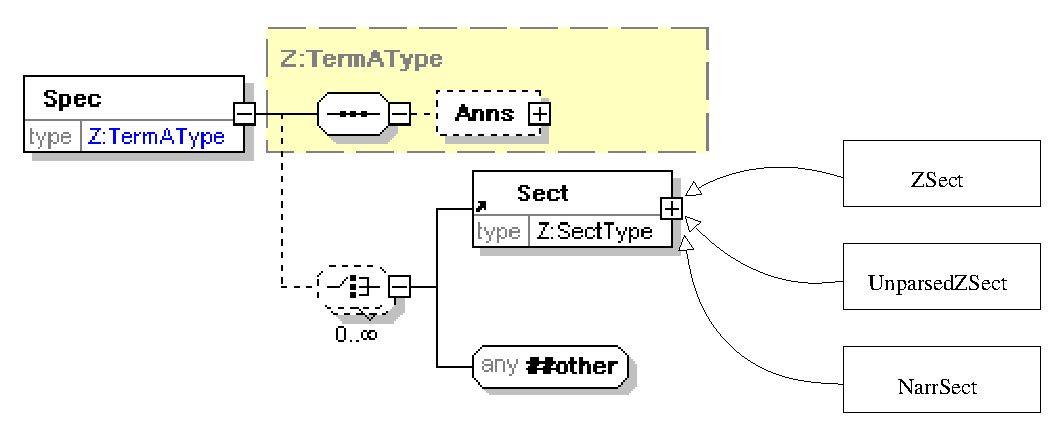
\includegraphics[width=0.9\textwidth]{specall2.eps}

\vspace{-3ex}
That is (in XML Schema):
\begin{footnotesize}
\begin{alltt}
<xs:element name="Spec">
    <xs:complexType> 
      <xs:complexContent>
        <xs:extension base="Z:TermA">
          <xs:choice minOccurs="0" maxOccurs="unbounded">
            <xs:element ref="Z:Sect"/>
            <xs:any namespace="##other" processContents="lax"/>
          </xs:choice> ...
\end{alltt}
\end{footnotesize}
\end{slide}

\begin{slide}
  \raisebox{20ex}{XML structure for a Z section.}
  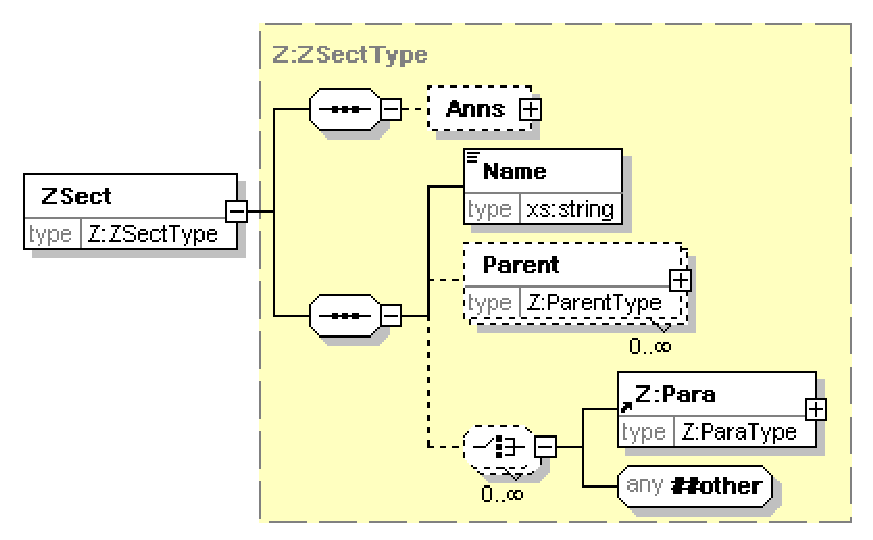
\includegraphics[width=0.6\textwidth]{zsect.eps}
\vspace{-6ex}

Example:
\begin{footnotesize}
\begin{alltt}
<Z:Spec>
  <Z:ZSect>
    <Z:Name>anonymous</Z:Name>
    <Z:Parent><Z:Word>definitions</Z:Word></Z:Parent>
    <Z:AxPara>...</Z:AxPara>
    <Z:NarrPara>
      <Z:Content>Here is some English commentary.</Z:Content>
    </Z:NarrPara>
    ...
  </Z:ZSect>
</Z:Spec>
\end{alltt}
\end{footnotesize}
\end{slide}


\begin{slide}
  \begin{center}
  XML structure for a axiomatic paragraph.\\
  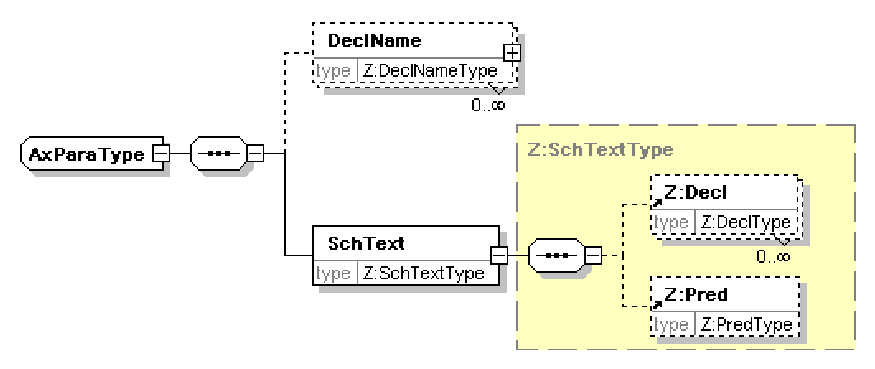
\includegraphics[width=0.8\textwidth]{axparatype.eps}
  \end{center}

Example:  \qquad $\mid p:PERSON$
\begin{footnotesize}
\begin{alltt}
<AxPara>
  <SchText Box="AxBox">
    <VarDecl>
      <DeclName> <Word>p</Word> </DeclName>
      <RefExpr> <RefName><Word>PERSON</Word></RefName> </RefExpr>
    </VarDecl>
  </SchText>
</AxPara>
\end{alltt}
\end{footnotesize}
\end{slide}


\begin{slide}
  \begin{center}
  A Quiz:  What Z generated this?\\
  \end{center}

\begin{footnotesize}
\begin{alltt}
<AxPara>
  <SchText Box="OmitBox">
    <ConstDecl>
      <DeclName> <Word>p</Word> </DeclName>
      <RefExpr> <RefName><Word>PERSON</Word></RefName> </RefExpr>
    </ConstDecl>
  </SchText>
</AxPara>
\end{alltt}
\end{footnotesize}
\vspace{16ex}
\end{slide}

\begin{slide}
  \begin{center}
  A Quiz:  What Z generated this?\\
  \end{center}

\begin{footnotesize}
\begin{alltt}
<AxPara>
  <SchText Box="OmitBox">
    <ConstDecl>
      <DeclName> <Word>p</Word> </DeclName>
      <RefExpr> <RefName><Word>PERSON</Word></RefName> </RefExpr>
    </ConstDecl>
  </SchText>
</AxPara>
\end{alltt}
\end{footnotesize}

Answer:  \qquad $p == PERSON$
\begin{verbatim}
         \begin{zed}
            p == PERSON
         \end{zed}
\end{verbatim}
\end{slide}



\begin{slide}
\begin{center}
The Challenge of Nested Identical Names.
\end{center}

Problem: If nested scopes declare the same name $X$, then
expressions inside the inner's scope cannot normally refer to the outer
$X$.
\begin{zed}
    [X] \\
\end{zed}
\begin{axdef}
    a : X
\where
    \exists X : \nat @ \# \{a\} = X
\end{axdef}

But type-checking must instantiate the generic operator $\#$,
so must introduce a reference to the outer $X$ (the $\# \{a\}$ becomes
$\#[X]\{a\}$). 

\textbf{Solution 1:} (Traditional) Rename the bound $X$.  No!  We want
injectivity. 

\textbf{Solution 2:} (Z standard) creates `suit-decorated' synonyms of 
  type names (e.g., $X\heartsuit$) and refers to those.  Not a general
  solution. 

\textbf{Solution 3:} (ZML) each declaration has an optional unique ID. 
  References can use those IDs.  (The ID/IDREF of XML Schema).
\end{slide}

\begin{small}
\begin{verbatim}
<GivenPara><DeclName Id="X.3"><Word>X</Word></DeclName></GivenPara>
\end{verbatim}
\end{small}
while an expression that references this $X$ can be marked up as:
\begin{small}
\begin{verbatim}
<RefExpr><RefName Decl="X.3"><Word>X</Word></RefName></RefExpr>
\end{verbatim}
\end{small}

  
\begin{slide}
\section{Conclusions and Questions}

\begin{itemize}
\item We have defined an XML mark-up for Z.
\item Design merges best features of: Z standard, \CADiZ, \Zeta.
\item Several small examples have been validated against the schema.
\item CZT: Elegant Java classes for Z have been generated from this XML
  schema.  We are now starting to integrate parser, type-checker, schema
  expansion, and translation to other notations.
\item We are seeking feedback and comments on the XML design, especially:
  \begin{enumerate}
  \item Annotations: in the XML (as here), or in a separate file?
  \item Non-standard paragraphs: quietly ignored (as here), or rejected?
  \item Unparsed fragments:  are these useful?  What granularity?
  \item Math Symbols: raw Unicode, or define symbolic names?
  \end{enumerate}
\end{itemize}
\end{slide}


\begin{slide}
\section{XML Mark-Up of a SMALL Example}
\newcommand{\NAT}{$\nat$}
\newcommand{\EXISTS}{$\exists$}
\begin{footnotesize}
\hrule
First we declare X to be a given set.
\begin{zed}
    [X] \\
\end{zed}
This axiomatic definition declares a:X, with the
  constraint: $(\exists X:\nat @ \#\{a\} = X)$
\begin{axdef}
    a : X
\where
    \exists X : \nat @ \# \{a\} = X
\end{axdef}
\hrule
\begin{alltt}
<NarrPara>
  <Content>First we declare X to be a given set.</Content>
</NarrPara>
<GivenPara>
  <DeclName Id="X.3"> <Word>X</Word> </DeclName>
</GivenPara>

<NarrPara>
  <Content>This axiomatic definition declares a:X, with the
  constraint: (\EXISTS X:\NAT @ #\{a\} = X)</Content>
</NarrPara>
<AxPara>
  <SchText>
    <VarDecl>
      <DeclName> <Word>a</Word> </DeclName>
      <RefExpr><RefName><Word>X</Word></RefName></RefExpr>
    </VarDecl>

    <ExistsPred>
      <SchText>
        <VarDecl>
          <DeclName> <Word>X</Word> </DeclName>
          <RefExpr><RefName><Word>\NAT</Word></RefName></RefExpr>
        </VarDecl>
      </SchText>
      <MemPred>
        <TupleExpr>
          <ApplExpr>
            <RefExpr>
              <RefName><Word>#</Word></RefName>
              <RefExpr>
                <RefName Decl="X.3"> <Word>X</Word>
                </RefName>
              </RefExpr>
            </RefExpr>
            <SetExpr>
              <RefExpr><RefName><Word>a</Word></RefName></RefExpr>
            </SetExpr>
          </ApplExpr>
          <NumExpr Value="1"/>
        </TupleExpr>
        <RefExpr><RefName><Word>=</Word></RefName></RefExpr>
      </MemPred>
    </ExistsPred>
  </SchText>
</AxPara>
\end{alltt}
\end{footnotesize}
\end{slide}
\end{document}
